\section{C++简介}

\begin{frame}\ft{C++起源}
  \begin{itemize}
  \item 
    \blue{产生时间:} 20世纪80年代\\[0.2in]
  \item 
    \blue{产生地点:}美国贝尔实验室\\[0.2in]
  \item 
    \blue{创始人:} Bjarne Stroustrup
  \end{itemize}
  \begin{figure}
    \centering
    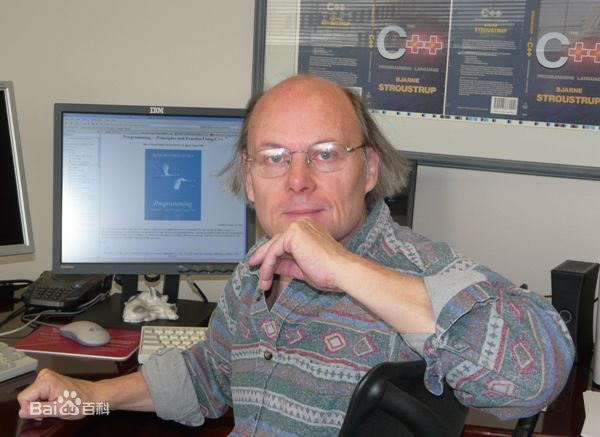
\includegraphics[width=2.5in]{slide01/images/Stroustrup.jpg}
  \end{figure}
\end{frame}

\begin{frame}\ft{C++发展}
  C++从最初的C with class,经历了从C++98、C++03、C++11、C++14再到C++17多次标准化改造,功能得到了极大的丰富,已经演变为一门集\red{面向过程、面向对象、函数式、泛型编程}等多种编程范式的复杂编程语言。
\end{frame}


\begin{frame}\ft{C++特点}
  C++融合了3种不同的编程方式:
  \begin{itemize}
  \item C语言代表的过程性语言
  \item C++在C语言基础上添加的类代表的面向对象语言(继承、封装、多态)
  \item C++模板支持的泛型编程。
  \end{itemize}
\end{frame}

\begin{frame}{C++的应用领域}
  \begin{itemize}
  \item 系统层软件开发
   \item 服务器程序开发
   \item 游戏、网络、分布式、云计算
   \item 科学计算
  \end{itemize}
\end{frame}

\begin{frame}{C++对C的增强}

  \begin{itemize}
  \item C是一个结构化语言,首要考虑的是如何通过一个过程,对输入(或环境条件)进行运算处理得到输出。
  \item C++首要考虑的是如何构造一个对象模型,让构造的模型能够契合与之对应的问题域,通过获取对象的状态信息得到输出或实现过程(事物)控制。
  \end{itemize}

  因此,C和C++的最大区别在于解决问题的思想不一样:
  \begin{itemize}
  \item C面向过程
  \item C++面向对象
  \end{itemize}

\end{frame}


\begin{frame}{C++对C的增强}
  C++对C的增强表现在六个方面:

  \begin{enumerate}
  \item 类型检查更为严格
  \item 增加了面向对象的机制
  \item 增加了泛型编程的机制(Template)
  \item 增加了异常处理
  \item 增加了运算符重载
  \item 增加了标准模板库(STL)
  \end{enumerate}
\end{frame}
